\chapter{Muon triggering and reconstruction}
\label{chap:xmuons}
\minitoc
\myepigraph{On est à une époque où toutes les connaissances sont
  accessibles si l’on s’en donne la peine : la difficulté est de
  trier, sélectionner, savoir où aller.}{Cédric Villani,
  in~\href{http://sciencespourtous.univ-lyon1.fr/cedric-villani-scientifiques-doivent-reprendre-main-partage-connaissances/}{\textit{Les
      scientifiques doivent reprendre la main sur le partage des
      connaissances}}, interview
  for Sciencespourtous.univ-lyon1.fr}





In this section we will see how CMS selects and processes collision
events delivered by the LHC.


The multipurpose experiments CMS and ATLAS have primarily been built to explore physics up to the \TeV\
scale, the Higgs boson discovery being one example~\cite{Aad:2015zhl}. Other high precision measurements are at stake in 
the electroweak sector, on the $t$ and $b$ quarks, as well as on QCD in extreme regimes. Some processes are extremely rare or not
discovered, yet every analysis needs a dedicated selection, from raw data to the latest stages of the analysis. One example from heavy ion
physics: the \PgUc, although well measured in $e^+e^-$, $pp$, $p\bar{p}$ and $pA$ collisions, is so suppressed that it is not observed at
this point in heavy ion collisions, and its nuclear modification is only expressed in the form of an upper limit on the total PbPb sample
(all centralities involved)~\cite{11-011}.


The \PgUc\ decaying to two
muons may be a simple signature, it is nonetheless a
detection challenge in a heavy ion environment. To get an idea of what
is the heavy ion multiplicity, we can for example consider that in the 5\% most
central PbPb events at $\snn\ =~2.76~\TeV$, CMS measured in 2010 a charged
hadron density per unit pseudorapidity of $dN_{\rm ch}/d\eta
\vert_{\eta=0} = 1612 \pm 55$ (\textit{syst.})~\cite{pbpbmult}. The
centrality in heavy ion collisions will be covered later
(Section~\ref{sec:centrality}), however, this simple measurement informs
us on the main difficulty encountered when measuring harder and rarer
probes: they are produced on top of an overwhelming background of
tracks that can cause the performance of the detector to degrade.% ,
% compared to what is seen in $pp$ collisions. Furthermore, the wealth
% of soft particles produced can decay to muons, and trying to analyse
% them all without selecting \textit{some} good quality muons and tracks
% would take an enormous amount of time and processing. 
For this reason,
a dedicated triggering strategy is indispensable to maintain good
event quality throughout analysis. 


The architecture and strategy of dimuon triggers for \PgU\ used in
this Thesis are detailed in Section~\ref{sec:triggers}. The muons
are reconstructed and further filtered offline, based on quality
requirements that are presented in Section~\ref{sec:muons}. In parallel of
most physics analyses, a more general event selection is needed, to
get an estimate of the luminosity of the $pp$ and PbPb
samples. Section~\ref{sec:evtsel} will present how the
number of hadronic events are counted in CMS, and how the global
selection is engineered to extract an information on the centrality of
the PbPb collision.% , on which the suppression of quarkonia is known to
% depend~\cite{torsten}.


\section{Triggers}
\label{sec:triggers}

% When the LHC delivers collision events to the experiments, the
% collision rate exceeds largely what each experiment can handle, and
% must be reduced to a reasonable level before data is stored and analysed. The
% CMS experiment has a sophisticated way to trigger on events of
% interest, using hardware and software based information combining all
% subdetectors.
% In the
% following, we will focus on the case of CMS, but the main ideas also
% work for other experiments.


% % The triggers are meant to select only events of interest out of all
% % the collisions produced in a LHC run. For every LHC fill, a number of
% % bunches of protons or ions are injected in the beams from, then ramped
% % up from E$_{SPS}$ = 450 \GeV\ to the desired beam energy. 

% % To perform collisions inside detectors, the beams are collimated and slightly diverted to end up on top of each
% % other at the Interaction Point (IP) of the detector. For CMS, the
% % LHC Interaction Point is called IP5. 
% In a typical proton proton run,
% the LHC beams are filled with more than one thousand proton bunches
% each. All bunches contain $N_{p} \approx 1\times 10^{12}$
% protons. Given the bunch spacing of 50 ns 

% high voltage is turned on in all the subdetectors of CMS. This
% procedure can be accommplished in a few minutes. From the point where
% 'stable beams' are declared, the full detector starts recording
% data. 


From its startup in 2009, the LHC has
gradually increased its instantaneous luminosity with time, almost
reaching the nominal value of $10^{34}$~cm$^{-2}$~s$^{-1}$, or 100 nb$^{-1}$~s$^{-1}$.
At the design luminosity of the LHC, the beam crossing frequency in
each experiment is 25 ns. Under these conditions, each experiment is
delivered up to 10$^{8}$ individual collisions. The input rate of
computing farms reconstructing data must be
reduced down to the order of less than 1 kHz, and several trigger levels are deployed in CMS
to achieve this task.




\subsection{The Level 1 Trigger}

% This collision rate is
% in fact reduced to 40 MHz at best, by three factors: the the progressive ramp up of beam
% performances in Run1, and by the filling scheme seen in
% Chapter~\ref{chap:xlhcms}, distributing approximately one third of
% colliding bunches to CMS. In the special conditions of a heavy ion
% run, the LHC filling scheme is 


The first trigger level of CMS, called L1~\cite{Dasu:2000ge}, is a
trigger system relying on hardware, meaning that it takes decisions
upon looking at raw data from the custom front end readout electronics.%  In a
% typical LHC $pp$ run of 2012, the collision rate in CMS could go as
% high as 500 MHz, which 

Its main challenge is to reduce the flow of events CMS
processes from the level of the collision rate (CR) down to a rate
sustainable by the HLT online processing computer farm. 

In the nominal settings of the LHC, the collision rate is 40 MHz; in 2012 when the instantaneous luminosity was
$2\times10^{33}$~cm$^{-2}$~s$^{-1}$ ($2$~nb$^{-1}$~s$^{-1}$), the collision rate was 13~MHz.

The decision to retain or reject an event has to be taken at every
bunch crossing, i.e. every 25 ns, under nominal conditions. The L1
trigger rate being limited by detector electronics, the trigger electronics are pipelined and
deadtimeless. This is important to treat in a
fast manner the Megabyte-sized raw events collected at every beam
crossing. Since new collision data arrive every 25 ns, the
processing of individual data cannot take more than 25 ns,
prohibiting the use of complicated algorithms. The pipelined architecture also requires that decisions
about one piece of an event are not based on data located somewhere
else in the event, not allowing for example a dimuon invariant mass to
be computed. The trigger based operations are simple arithmetic ones,
using lookup tables addressing segments of the subdetectors in broad
$\eta-\phi$ regions.

The size of the detector cavern and the distance to the trigger electronics
places a time limit of 3.2 $\mu$s on L1 trigger processing for a
single event. Under nominal design, this corresponds to 128 beam
crossings. The longest data processing time comes from Muon Barrel
drift chambers, whose drift time takes 400 ns before full signal
collection. The 3.2 $\mu$s time restriction also means that the
trigger cannot include ECal preshower or Tracker data in the decision.

The remaining subdetectors (ECal and HCal Barrel plus Endcaps, HF, Muon RPC,
CSC and DT) read out event data separately. The architecture of the L1 trigger, described here, is summed up in
Figure~\ref{fig:L1arch}. The readout data sent to the
Data Acquisition system (DAQ) is bundled in trigger
\textit{primitives}.


The Electronic Calorimeter (ECal), the Hadronic Calorimeter (HCal) and
Hadron Forward calorimeters (HF) record energy that is summed in 'trigger towers' directly from
calorimeter cell energies. The Regional Calorimeter Trigger (RCT)
identifies electron, photon, tau, jet candidates and $E_{T}$ sums, forwards
it to the Global Calorimeter Trigger (GCT) which is in charge of sorting the
top 4 candidates of each type and calculate total $E_{T}$ and missing
$E_{T}$. The information is then sent to the Global Trigger.

Since muons are minimally ionising the calorimeters, the quiet
$\eta-\phi$ calorimeter regions can be mapped by the RCT, to be
transmitted to the Global Muon Trigger (GMT) for muon isolation cuts.
\\
Each muon subdetector has its own trigger
logic.

Resisitve Plate Chambers (RPC) use a projective pattern comparator to form trigger segments from
lighting RPC strips. These segments can be connected together to
find tracks and calculate their \pt. Since RPC overlap with Cathode
Strip Chambers (CSC), the
RPC logic is allowed to communicate with the CSC trigger system, which
improves the resolve of ambiguities when two muons hit the same CSC. 

The CSC form Local Charged Tracks (LCT).  The LCTs are
assigned a \pt\ and a quality
bit, which are sent to the CSC Track Finder (CSCTF) to sort the best 3
LCTs sector by sector\footnote{A sector is composed of nine CSC chambers.}. The CSCTF further combines the LCTs into full muon tracks, and
in the region where the CSC overlap with the Drift Tubes (DT), both CSCTF and Drift Tube track finders (DTTF) exchange segment information to improve themselves.


\begin{figure}[h]
\begin{center}
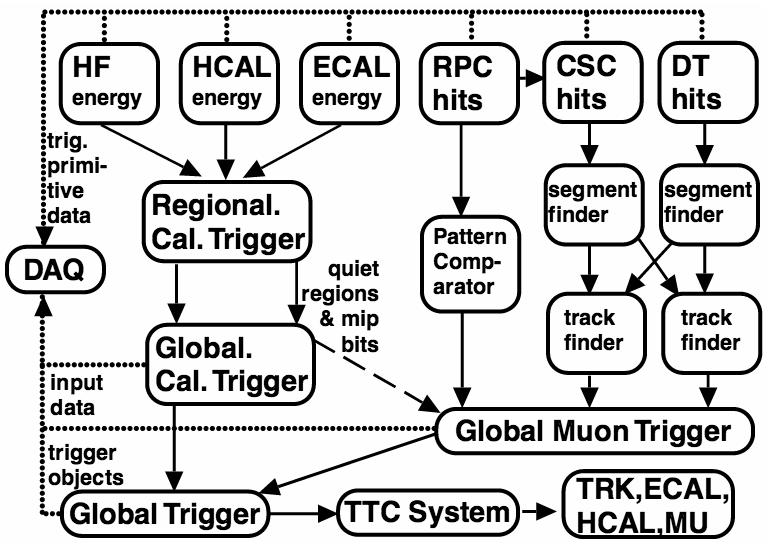
\includegraphics[width=0.83\textwidth]{Chapters/xLHCMS/L1Trigger.png}
\caption{Overview of the L1 Trigger architecture~\cite{Dasu:2000ge}.} 
% Personal compilation for Scomparin~\cite{scomparinlhcp2014}.}
\label{fig:L1arch}
\end{center}
\end{figure}


In the barrel, the DT uses a track identifier to match aligned hits in
each DT layer into segments matched to a single superlayer (SL). The track segments' positions and angles
are correlated when their $\phi$ coordinate coincide, and the best two
combinations are sent to the DTTF, merging them into full muon tracks
assigned with a \pt.

The GMT later receives the best muon tracks from RPC, CSC and DT track finders, sorts them by quality, and the best four muon candidates are sent to the Global Trigger (GT).

Based on GCT and GMT signals, the GT accepts muon and calorimeter candidates, sending L1 Trigger decisions to the Timing Trigger
and Control module (TTC) which then communicates back with subdetectors to initiate the readout. The L1 decisions are
logical \textit{trigger paths} defined by user and requesting for example:
\begin{itemize}
\item[-] The presence of up to four muon candidates, eventually close or far from each other in $\eta-\phi$, above a
  \pt\ threshold, in $\vert\eta\vert < 2.4$;  %, and possilbly with confirmed matching in overlapping CSC-DT regions and/or CSC-RPC regions;
\item[-] The firing of up to four calorimeter towers above e.g. 30 \GeV\ by electron/photon candidates, in
  $\vert\eta\vert < 2.5$;
\end{itemize}

The full list of L1 triggering possibilities is detailed in Sections 2.2 and 2.3
of~\cite{Dasu:2000ge}. The above two examples can be used to identify
Standard Model physics processes, such as $\PgU\to\mu\mu$,
$Z^{0}\to\mu\mu$, or $H\to\gamma\gamma$, $H\to 4l$, etc. In the same time, some of the 128 L1 trigger bits available can
be used to implement global event measurements (geared towards a luminosity estimation), or efficiency measurements (RPC
efficiency while triggering on CSC-DT and vice versa).

The LHC will operate at least up to 2035~\cite{commissioning}. In this
time, additional computing nodes can be added to the trigger
system, as well as network technologies and electronics can
evolve. For these reasons, although the event builder and event filter
can perform at 100 kHz (design
capabilities~\cite{Dasu:2000ge}), the L1 trigger output rate capability was in 2012
bridled at 50 kHz. 


The LHC filling scheme for heavy ions is different to that of $pp$ collisions and as a result, the beam crossing time
changes to 200 ns. The collision rate is smaller, which is good for the triggers since high multiplicity events
are large (the raw event data can exceed 5 Mb). Separately of L1 decisions, the Pixel detector, which is closest to
the beam pipe, is under high illumination at every moment. To stay in the bandwidth of the pixel readout
system, the L1 output rate is generally limited to 5$\sim$10 kHz.


The output L1 and readout data are sent to the High Level Trigger for refined filtering.



\subsection{The High Level Trigger}

The second and third levels of the CMS trigger system are called the High Level Trigger (HLT). The HLT relies on
software algorithms running on an online computing farm of 13,000 commercial CPU cores~\cite{Trocino:2014jya}. The raw output data accepted at L1 is streamed to a subset of the computer farm (L2) which
is then sent to the other subset (L3) for further filtering. The data reduction rate, from the L1 output to the HLT
output, is of the order of 10$^{3}$, i.e., the HLT output rate is of the order of 100 Hz to 1 kHz.  The size and processing time of events is again
an important limiting factor, especially in the case of heavy ion
data, where the multiplicity of tracks is huge. In order to maintain
a smooth transfer to the Tier0 storage system, both the L1 and HLT
rates have to be kept within the bandwidth (of the order of 1 Gb/s).


The HLT relies on more refined algorithms than L1 to decide if the
event should be kept. The
$\sim$ 200 paths of a total typical HLT menu are run in parallel in the computing farm, using data from all subdetectors to
proceed to a first reconstruction of the physical objects (muons, electrons, taus, missing energy). This online reconstruction
is a streamlined copy of the offline reconstruction, and kept only to regions of the event where the physical
object of interest is defined, to save computing time.
% The Level-1 Trigger combines information of ECal and Muon
% subdetectors, but not of the tracker, constrained to a longer readout
% time to avoid overflow.

The various HLT paths can be seen as non exclusive streams, meaning that all data accepted under a certain condition at
L1 \textit{seeds} one or many HLT paths. Several HLT paths can
originate from the same L1 seed. 

In the following, I will focus on muon trigger sequences: other
reasonings apply to $e$/$\gamma$ triggers, as their L1 seeds originate
from other parts of CMS. 


 The HLT path used in the case of \PgU\ decaying to two
muons is a dimuon HLT path, seeded by a dimuon
L1 seed. A HLT path is a sequence of reconstruction and filtering
modules, developed by the user or the analysis group, for the needs of
a physics analysis or an efficiency estimation. The HLT path sequence
% for muons is usually constructed in the following way:
% \begin{itemize}
% \item[-] the L1 seed is opened and a prescale $k$ is applied, meaning
%   that the path processes one event out of $k$,
% \item[-] 
% \end{itemize}
begins with the L2 reconstruction sequence, using the L1 seed and
digitised readout from the CSC, RPC and DT to construct
a \textit{standalone} (STA) muon, based solely on muon detector
informations. The STA muon is of usually poor resolution. The L2
reconstructed object is optionally filtered for some quality
requirements (on the muon chamber hits) or kinematics ($\eta, \pt$
cuts). If the event does not pass the filtering step, it is discarded
and will not be sent to L3.

The L3 step uses the L2 output STA muon as seed to an outside-in
reconstruction, involving the digitised data read out of the pixel
detector and silicon trackers. The reconstruction sequence can either
stop here and proceed to final filtering, or extend to include an
inside-out refitting of the muon track and STA global object.
Filtering cuts on the L3 level resemble that of L2, to the exception
that the resolution is improved with the input of the tracker
information, and cuts can also apply to the tracker part. Additional cuts on the four-momentum of a dimuon system
can be computed, for example on impact parameter, mass or transverse momentum.




In the preparation of a physics analysis, one should always develop at
least one control trigger, dedicated to efficiency studies of the
various trigger steps involved the `physics' trigger(s). In the case
of dimuon triggers, one way to assess the various levels of
reconstruction is to prepare single muons triggers essentially
following the same selection at L2 and L3 as the dimuon trigger. One
can also develop a L2 single muon trigger and a L3 single muon trigger
to understand the efficiency of the matching of L2 and L3 objects.


In cases when the rate expected for a certain trigger (for physics or
efficiency) gets too high, either because of the collision rate or
because of the loose requirement of the trigger, one can apply a
prescale factor $k$, such that at HLT processing, only one event out
of $k$ events firing the L1 seed will be processed. 

In the following, we will see in what conditions the detector was
operated for the 2011 PbPb collision run.





% In $pp$ runs, starting 2012, about half of the events processed at HLT are stored to tape for further processing. This
% is \textit{data parking}. An interesting explanation of the motivations for data parking can be found in~\cite{strassler}.




% The HLT is a software based trigger. It processes events using readout
% information from various subdetectors, using separate logical paths that are
% built by the user to suit its analysis needs. The total output of the
% HLT must not exceed 1 kHz. 

% In an ongoing physics run, all HLT trigger paths work at the same time, and
% record separate events at separate rates. The sum of all paths is
% called the trigger 'menu'. Usually, there is a menu per analysis
% object: in the case of heavy ion collisions in CMS, we distinguish
% muon based physics analyses from other types of heavy ion analysis,
% based on jets or the full minimum bias event, for example. In turn,
% the muon based menu contains single muon and double muon paths
% dedicated to the analysis of muon objects in heavy ion collisions.


% While the L1 will reduce the rate of recorded events to include only
% interesting events (e.g. double muon events) using raw readout
% information, the HLT will further reduce the rate of analysed events,
% using cleaner particle signatures (e.g. displaced muons, or good
% quality muon tracks). It can also make more accurate cuts on the kinematic and
% topology of the signature. 



\subsection{Settings for the 2011 PbPb run}
\label{sec:HiRates}

To measure hard probes such as quarkonia in PbPb collisions, the requirement that a hadronic event occurred is
important to remove ultra-peripheral events, beam-gas interactions and
other beam remnants. This is implemented at level-1, with the
requirements that enough energy deposits in both sides of the HF are coincident with the hard
event of interest. This global event selection will be further
detailed in Section~\ref{sec:evtsel}, and the rest of the subsection
is dedicated to beam and detector settings for the 2011 PbPb data
taking, with a focus on the dimuons of interest in this \PgU\ analysis.


In a typical heavy ion LHC fill of 2011, for example fill 2328, the filling scheme was:
\begin{equation*}
  \verb?200ns_358b_356_336_0?
\end{equation*}

This means that the bunch spacing was 200 ns, 358 bunches were
injected, 356 were distributed to IP1/5 (i.e. ATLAS and CMS), 336 were
distributed to IP2 (ALICE), and none to LHCb.
At 200 ns bunch spacing, the L1 and the detector electronics face a
collision rate of 5 MHz, which is well below the limits of what the
hardware trigger can handle. 

Under these conditions, the L1 trigger is set to handle an
instantaneous luminosity scenario of $10^{28}$~cm$^{-2}$~s$^{-1}$
($10$~mb$^{-1}$~s$^{-1}$) maximum.

Again using the example case of LHC fill 2328 (CMS run number 182572),
which is comparable to other runs of the 2011 data taking,
the luminosity at starting time of the run was $470\times 10^{27}$~cm$^{-2}$~s$^{-1}$
($4.7$~mb$^{-1}$~s$^{-1}$). The L1 output rate was 1483 Hz, indicating
that only a small amount of filtering would be needed at further
levels. The run lasted for approximately seven hours, with an
instantaneous luminosity of $153\times 10^{27}$~cm$^{-2}$~s$^{-1}$
($1.53$~mb$^{-1}$~s$^{-1}$) at the time of the beam dump. The
integrated luminosity delivered to CMS for this run was 5.76~\invmub,
representing about 3\% of the total luminosity delivered to CMS in the
PbPb run of 2011. The integrated luminosity recorded by CMS was 5.64
\invmub, which represents a 98\% data taking efficiency.  % In the case of the dimuon trigger used at L1, named 



The L1 seeds for our dimuon triggers are `open', in the sense that
they do not cut on the \pt\ of the muons or that of the dimuon, and retain every event
identified as a dimuon candidate by the GMT and GT. In our case,
calorimeter based isolation is not used. The L1 seed is called
\verb?L1_DoubleMuOpen_BptxAND?. The BPTX suffix is here to denote that
the dimuon L1 signal is coincident with the signal rise time of beam
position monitors (Beam Position and Timing for LHC eXperiments, BPTX~\cite{4774822}) . This \textit{gating} was implemented
during the run to remove the cosmic ray contribution to the L1 dimuon rate.

% We shall see in Section~\ref{sec:muons} some
% aspects of the performance of this trigger of the muon reconstruction at low-\pt.
In the same run as considered previously (number 182572), the L1 rate
for the path \verb?L1_DoubleMuOpen_BptxAND? started at about 95 Hz,
down to 35 Hz at dump time. The rate \vs. time can be seen in
Figure~\ref{fig:rate2011} (left).

\begin{figure}[h]
\begin{center}
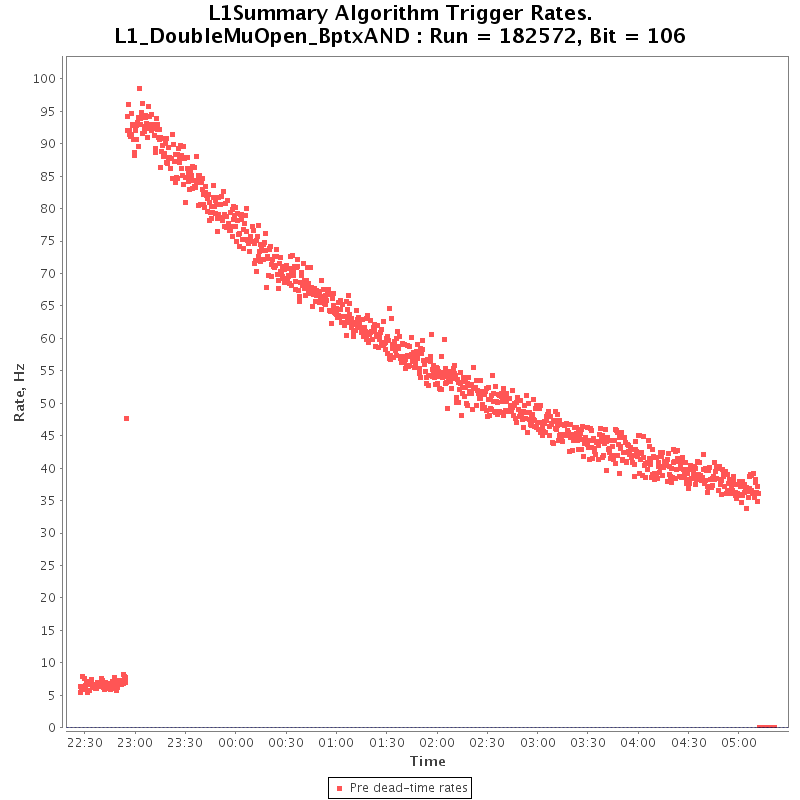
\includegraphics[width=0.46\textwidth]{Chapters/xLHCMS/L1rate_2011.png}
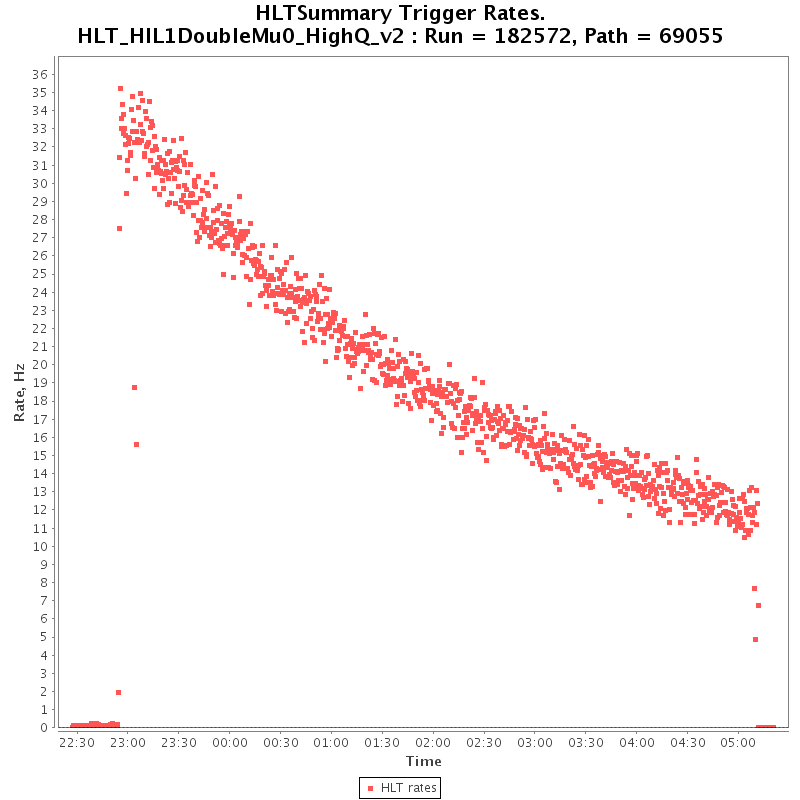
\includegraphics[width=0.46\textwidth]{Chapters/xLHCMS/HLTrate_2011.png}
\caption{Rates of the open dimuon trigger in the 2011 PbPb run. Left:
  rate of L1\_DoubleMuOpen\_BptxAND; Right: rate of HLT\_HIL1\_DoubleMu0\_HighQ.} 
% Personal compilation for Scomparin~\cite{scomparinlhcp2014}.}
\label{fig:rate2011}
\end{center}
\end{figure}


Thanks to the low rate at L1, a reasonable HLT rate could be
maintained in the muon `menu' at HLT. Four dimuon HLT paths based on
\verb?L1_DoubleMuOpen_BptxAND? were configured, all of them
unprescaled (i.e. no L1 event is skipped, $k$ = 1). Their
names are:
\begin{eqnarray*}
 & &\verb?HLT_HIL1_DoubleMu0_HighQ?\\
 & &\verb?HLT_HIL3_DoubleMuOpen?\\
 & &\verb?HLT_HIL2_DoubleMu3?\\
 & &\verb?HLT_HIL3_DoubleMuOpen_Mgt2_OS_NoCowboy?
\end{eqnarray*}

The four HLT paths have different levels of filtering, as well as
rate, and efficiency.
\\
The HighQ suffix in the first path is a Level-1 quality bit cut. The
L1 muons are assigned a quality bit depending on their status in muon
subdetectors; in this case, the quality bits of L1 muons are the
following:
\begin{itemize}
\item[bit 0] \textbf{(rejected)} - Empty muon candidate;
\item[bit 1] \textbf{(rejected)} - Halo muon for alignment;
\item[bit 2] \textbf{(rejected)} - Very Low Quality Type 1, skipped in
  single and di-muon triggers;
\item[bit 3] \textbf{(rejected)} - Very Low Quality Type 2, skipped in
  single muon triggers;
\item[bit 4] \textbf{(rejected)} - Very Low Quality Type 3, skipped in
  di-muon triggers;
\item[bit 5] \textbf{(kept)} - Candidate muon detected in DT and/or CSC, but not
  confirmed in RPC;
\item[bit 6] \textbf{(kept)} - Candidate muon detected in RPC, but not
  confirmed in DT and/or CSC;
\item[bit 7] \textbf{(kept)} - Candidate muon detected in RPC and DT, or in
  RPC and CSC.
\end{itemize}

The `HighQ' decisions are highlighted in bold, to exclude halo muons
used for alignment and calibration, as well as very low quality or empty muon
candidates.

\verb?HLT_HIL3_DoubleMuOpen? has basically no filtering specific to L2 and L3;
however the online reconstruction chain is done up to L3. Such a
trigger can be useful in express streams (i.e. immediate
reconstruction to check the quality of recorded data), or for timing
of the full reconstruction chain.


The L2 trigger \verb?HLT_HIL2_DoubleMu3? has a cut on each L2 muons
of \pt=3 \GeVc. This trigger is not used in quarkonia, as it would
discard a lot of events in the forward region (where the \pt\ reach of
\Jpsi\ can be extended to zero, interesting if one wants to measure charmonium
regeneration in heavy ions). It is however a useful trigger for the Z
boson, since the rate is reduced compared to the open trigger.

The L3 trigger \verb?HLT_HIL3_DoubleMuOpen_Mgt2_OS_NoCowboy? attempts
to remove events where muons bend towards each other, in the x-y
plane. Such dimuon events are called `cowboys', and can have a lower
efficiency, since they would often cross each other in the first muon
station at low \pt, lowering the track matching efficiency. This
trigger also cuts on opposite sign muon pairs, with an invariant mass
above 2 \unitMass.

Typical HLT rates of the 2011 PbPb runs are taken from run 182572 and
presented in Table~\ref{tab:rates2011}. The table reports the maximal rate
(at the beginning of the physics run), the average rate, and the
fraction of the total HLT output (computed by dividing the average
rate and the average HLT total rate of 239 Hz).

\begin{table}[h]
  \begin{center}
    \begin{tabular}{|c|c|c|c|}
      \hline
      HLT path & Max (Hz) & Avg. (Hz)& \% of total
      HLT\\
      \hline
      \hline
      \verb?HLT_HIL1DoubleMu0_HighQ?& 35 & 18 & 7.5\%\\
      \verb?HLT_HIL3_DoubleMuOpen?  & 23 & 12 & 5\%\\
      \verb?HLT_HIL2_DoubleMu3?     & 11 & 5 & 2\%\\
      \verb?HLT_HIL3_DoubleMuOpen_Mgt2_OS_NoCowboy?& 7 & 3 & 1.25\%\\
      \hline
    \end{tabular}
    \end{center}
  \caption{HLT rates for dimuon triggers in the PbPb data taking of
    2011. Columns report the total rate, average rate, in Hz,
    and the fraction of total HLT rate.}
\label{tab:rates2011}
\end{table}

These triggers are meant for physics and need to be backed up with
efficiency triggers. The list of active single muon triggers for
efficiency studies is reported here:

\begin{eqnarray*}
  & &\verb?HLT_HIL3_Mu3?\\
  & &\verb?HLT_HIL2_Mu3_NHitQ?\\
  & &\verb?HLT_HIL2_Mu7?\\
  & &\verb?HLT_HIL2_Mu15?\\
\end{eqnarray*}

Each single muon trigger starts with a L1 seed
called~\verb?L1_SingleMu3_BptxAND?. This seed requires that each L1
candidate has a \pt\ of more than 3 \GeVc. 
\\
The L3 path~\verb?HLT_HIL3_Mu3? is constructed along requiring at
every level that the L2 or L3 object has a \pt\ above 3 \GeVc.


The L2 path~\verb?HLT_HIL2_Mu3_NHitQ? applies a prefilter on the L1
object prior to reconstruction, requesting the L1 to contain at least
one muon chamber hit. The L2 reconstruction
sequence further requires that the L2 muon track is reconstructed from at least 2 hits.


The L2 path~\verb?HLT_HIL2_Mu7? does not apply strict requirements on
the number of hits further than what the L2 reconstruction sequence
asks for, but the \pt\ of the L2 muon has to exceed 7 \GeVc\ to pass,
which is useful in $Z$ boson efficiency studies.%  This trigger could
% also be used in $W$ boson analyses.


The L3 path~\verb?HLT_HIL2_Mu15? has the strongest \pt\ requirement, of
15 \GeVc. This requirement is useful to record muons coming from Z bosons, as well as W bosons.


The rates of single muon paths are reported in
Table~\ref{tab:murates2011}. The table reports the max rate
(at the beginning of the physics run), the average rate, and the
fraction of the total HLT output (computed by dividing the average
rate and the average HLT total rate of 239 Hz).

\begin{table}[h]
  \begin{center}
    \begin{tabular}{|c|c|c|c|}
      \hline
      HLT path & Maximum rate (Hz) & Average rate (Hz)& \% of total
      HLT\\
      \hline
      \hline
      \verb?HLT_HIL3_Mu3?& 99 & 51 & 21\%\\
      \verb?HLT_HIL2_Mu3_NHitQ?& 97 & 50 & 21\%\\
      \verb?HLT_HIL2_Mu7?& 26 & 13 & 5.5\%\\
      \verb?HLT_HIL2_Mu15?& 9.5 & 4 & 1.8\%\\
      \hline
    \end{tabular}
  \end{center}

  \caption{HLT rates for single muon triggers in the PbPb data taking of
    2011. Columns report the total rate, average rate, in Hz,
    and the fraction of total HLT rate.}
\label{tab:murates2011}
\end{table}



\subsection{Monitoring of the 2013 \texorpdfstring{$pp$}{pp} run}
\label{sec:pp2013}

% The $pp$ and $p$-Pb run of 2013 were recorded with very close
% requirements to that of the PbPb run. 
I have participated to the $pp$ and $p$Pb data taking run of 2013 and
have done some service work on the monitoring of the muon
triggers. Some of these triggers are used to record the $pp$ data used in 
this thesis.

The proton-proton run of 2013, at the centre-of-mass energy of $\s =
2.76~\TeV$, was recorded from LHC fill 3555 to 3564, between February,
11$^{\rm th}$, 2013, and February, 14$^{\rm th}$, 2013.


In the following Table~\ref{tab:runconditions_pp}, the run conditions
of the $pp$ data taking are presented: LHC Fill, CMS run number,
initial instantaneous luminosity, L1 average accept rate, HLT average
accept rate. The
collision rate varied from 100 kHz to 5 MHz, because of the increase
bunch filled in the LHC for each fill.


\begin{table}[h]
  \begin{center}
    \begin{tabular}{|c|c|c|c|c|}
      \hline
      LHC Fill & CMS run & Max $\mathcal{L}$ ($\times
      10^{30}$~cm$^{-2}$~s$^{-1}$)& L1 rate (kHz) & HLT rate (kHz)\\
      \hline
      \hline
      3555 & 211739, 211740& 4 & 14 & 0.72 \\
      3556 & 211752& 55 & 28.5 & 1.09\\
      3557 & 211760& 123 & 44 & 0.96\\
      3558 & 211765& 141 & 73 & 1.60\\
      3559 & 211765& 135 & 41 & 1.55\\
      3560 & 211797& 143 & 54 & 1.75\\
      3564 & 211831& 117 & 53 & 1.84\\
      \hline
    \end{tabular}
  \end{center}
  \caption{Run conditions for the $pp$ data taking in 2013, at \s\ =
    2.76 \TeV.}
\label{tab:runconditions_pp}
\end{table}

The total HLT rate is composed at $\approx$ 30\% of data reserved for alignment
and calibration purposes. The actual rate of physics triggers did not exceed 1
kHz.


The muon triggers deployed during the 2013 runs contain equivalents to
the 2011 paths, as well as new additions, overlapping with the `jet physics'
menu. The list of L1 muon and dimuon paths active for
quarkonia and electroweak probes\footnote{Paths related to B mesons,
  jets and ultraperipheral quarkonia are not included in the list.} during the run is detailed below:

\begin{eqnarray*}
& & \verb?L1_SingleMu3? \\
& & \verb?L1_SingleMu7? \\
& & \verb?L1_SingleMu12? \\
& & \verb?L1_DoubleMuOpen_BptxAND? 
\end{eqnarray*}

The HLT paths seeded by these L1 paths are reported next:

\begin{eqnarray*}
& & \verb?HLT_PAMu3? \\        
& & \verb?HLT_PAMu7? \\        
& & \verb?HLT_PAMu12? \\       
& & \verb?HLT_PAL1DoubleMuOpen? \\
& & \verb?HLT_PAL1DoubleMu0_HighQ? \\
& & \verb?HLT_PAL2DoubleMu3? \\
\end{eqnarray*}


The single muon paths were seeded with the L1 path of same \pt\
threshold, and the double muon paths all originate from the only
double muon L1 seed.


% For a LHC fill with high L1 rate, e.g. fill 3560, the CMS run 211797
% reports the following HLT rates and L1 rates,


Typical HLT rates of the $pp$ runs are taken from run 211797 and
presented in Table~\ref{tab:rates2013}. The table reports the max rate
(at the beginning of the physics run), the average rate, and the
fraction of the total HLT output (computed by dividing the average
rate and the average HLT total rate of 1.751 kHz) of muon and dimuon paths.

\begin{table}[h]
  \begin{center}
    \begin{tabular}{|c|c|c|c|}
      \hline
      HLT path & Maximum rate (Hz) & Average rate (Hz)& \% of total
      HLT\\
      \hline
      \hline
      \verb?HLT_PAMu3?   &763 &498 &29 \%\\
      \verb?HLT_PAMu7?   &69 & 40&2.2 \% \\
      \verb?HLT_PAMu12?   &7 &3.6 & 0.2 \% \\
      \verb?HLT_PAL1DoubleMuOpen?  &100 &58 & 3.3 \% \\
      \verb?HLT_PAL1DoubleMu0_HighQ? &49 &29 & 1.7 \% \\
      \verb?HLT_PAL2DoubleMu3?  &16 &9 & 0.5 \% \\
      \hline
    \end{tabular}
    \end{center}
  \caption{HLT rates for dimuon triggers in the PbPb data taking of
    2011. Columns report the total rate, average rate, in Hz,
    and the fraction of total HLT rate.}
\label{tab:rates2013}
\end{table}

We can see in Table~\ref{tab:rates2013} that the total muon rate
accounts for about 36 \% of the total recorded data. While the average
HLT output rate is high, let us recall that about 30 \% of the HLT rate
does not go to the physics-oriented reconstruction, and is used for
alignment and calibration of subdetectors.
Additionally, the CPU load was kept reasonable throughout the
processing, at an average of 27 \% of the total available bandwidth,
benefitting from the small number of HLT paths processed and the small
size per event.

In the muon dataset, at an average total rate of 600 Hz, the average
file size is 100 kilobytes per event. This information can be
retrieved from web based monitoring servers recording statistics on
data quality and processing rate.

At the beginning of a $pp$ run, the total muon rate (dominated by the
single muon triggers) could go up around 800 Hz alone. This is
high, however, looking at the file size per event, we can compute the
bandwidth occupied by raw muon data in the HLT stream, which is 80 Mb
per second. This is well below the limits of the HLT stream to storage centers
(on the order of 1 Gb/s) and gave us confidence in maintaining high
rates.



In the muon trigger HLT menu, the fact that various HLT paths come
from a common L1 seed will induce correlations between the firing of
HLT paths. For example, a muon of \pt\ = 9 \GeVc\ will fire the L1
seed \verb?L1_SingleMu3?, which would then fire the HLT paths
\verb?HLT_PAMu3? and \verb?HLT_PAMu7?, but not the path
\verb?HLT_PAMu12?.



It is important to know the correlations in our triggers, since one of
the triggers, \verb?HLT_PAMu3? dominates the total muon HLT rate; if
the rate gets high at the beginning of a new run, we want to be able
to act fast and decide what prescale to apply to this trigger. In
doing so we can also know what the effect of the prescale would have
on the rates of the rest of the triggers (\verb?HLT_PAMu7?,
\verb?HLT_PAMu12?, but also dimuon triggers and jet+muon triggers).


To investigate the effect of the correlation, one can construct a
correlation matrix between all muon paths including the ones using
jets, which would help to map out all the overlaps between triggers
firing on muons. Figure~\ref{fig:correlationHLT} shows such a matrix.

The correlation matrix shown was computed for the run 211752, in which
the \verb?HLT_PAMu3? path produces 69.2 \% the total rate. If we look
back at Table~\ref{tab:runconditions_pp}, we can see that run 211752
came in one of the first fill, when the luminosity of the proton beams
was being ramped up progressively by the accelerator teams. To
anticipate the rate of muon triggers at full luminosity (e.g. in runs
posterior to 211752, cf. Table~\ref{tab:runconditions_pp}), I
have produced this correlation matrix. 

% A prescale factor $k = 3$ had just been applied to
% the \verb?HLT_PAMu3? path at the beginning of this run, to reduce its
% impact on the total muon rate\footnote{This is the sum of muon HLT
%   rates, not to be confused with the total HLT rate!}, from 
% 98 \% to 69.2 \%. The dimuon paths are somwehat decorrelated from
% others, which is expected since their firing requires two L1 muons
% instead of one. 




To get a good idea of how triggers overlap, one can look at the second
column of Figure~\ref{fig:correlationHLT} to read what fraction of
\verb?HLT_PAMu3? firings (which dominate, as said above) is shared
with other triggers. This is relevant since \verb?HLT_PAMu3? dominates
the total muon rate, all other correlations having smaller
effects. The largest overlap of \verb?HLT_PAMu3? is with the jet + muon path 
\verb?HLT_PAMu3_PFJet20?, and is of 8.3 \%. For a predictive total
muon rate of 800 Hz, the \verb?HLT_PAMu3? rate would be 550 Hz. With an
overlap of 8.3 \% of \verb?HLT_PAMu3? with \verb?HLT_PAMu3_PFJet20?, we obtain
that the dominant \verb?HLT_PAMu3? rate would be responsible for 45.7
Hz out of the \verb?HLT_PAMu3_PFJet20? rate. This turned out to be
close to the rate of \verb?HLT_PAMu3_PFJet20? in
consecutive runs at nominal luminosity (for example,
\verb?HLT_PAMu3_PFJet20?(run 211797) = 49.5 Hz), confirming that our
predictions were accurate.


\begin{figure}[h]
\begin{center}
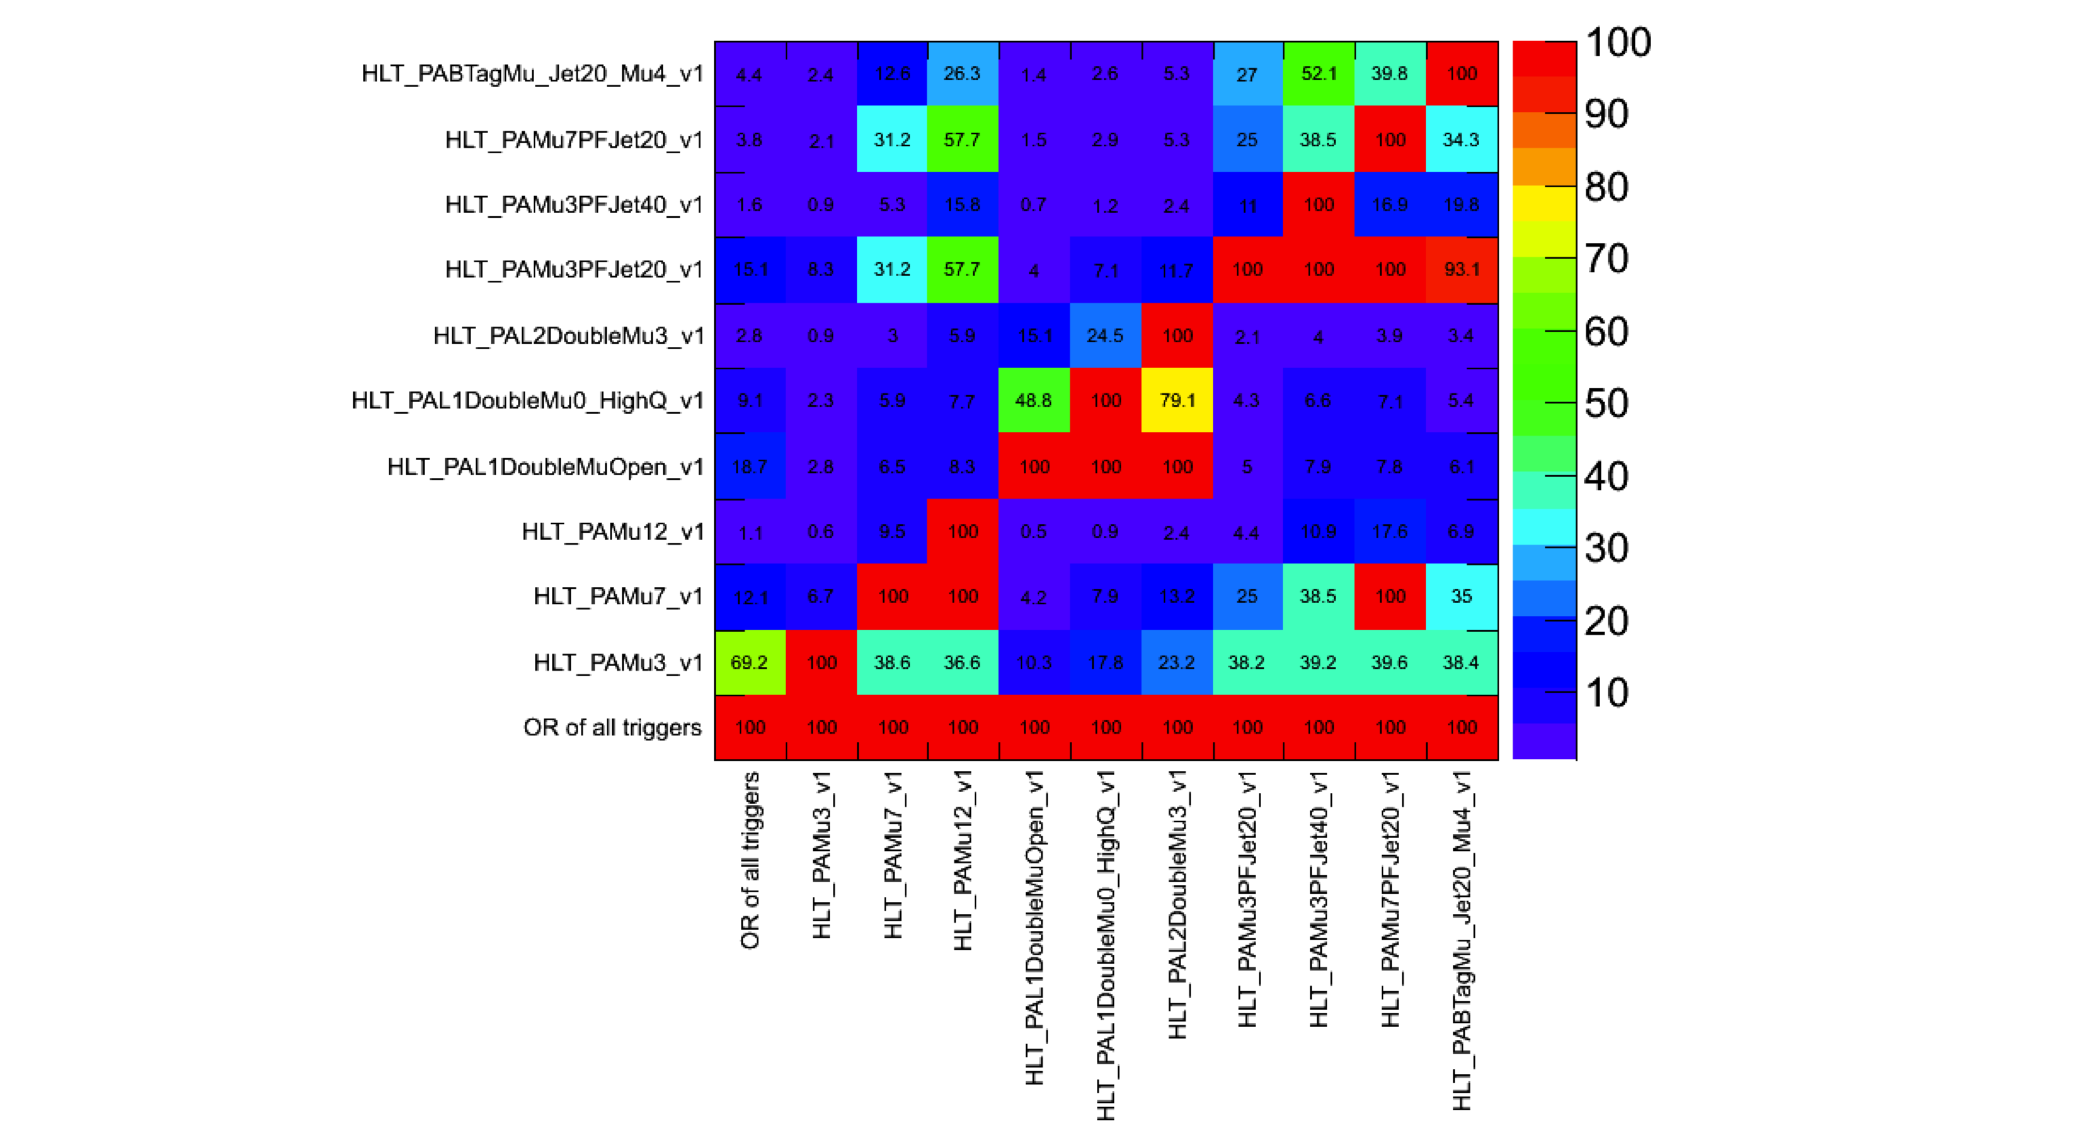
\includegraphics[width=1.1\textwidth]{Chapters/xLHCMS/Correlations.png}
\caption{Correlation matrix of HLT muon rates, used to compute the
  overlap between paths sharing common L1 seeds. The dominant rate of
  HLT\_PAMu3 is prescaled by a factor three.} 
% Personal compilation for Scomparin~\cite{scomparinlhcp2014}.}
\label{fig:correlationHLT}
\end{center}
\end{figure}


\vspace{0.5em}
\begin{center}
  \fbox{
    \parbox{0.9\textwidth}
    {\textsf {In this section we have seen how collision data gets
        stripped down to only the subset of events of interest for
        further analysis, thanks to the L1 and HLT trigger levels of
        CMS. The data has to be passing trigger 
        filtering requirements that can be organised in three levels,
        along the various reconstruction sequences. In 2013, high muon
        rates above the 100 Hz level were 
        affordable for analysis and were dominated by
        efficiency-oriented trigger paths. This ensures a large $pp$
        sample for physics and for efficiency studies, important to
        know the suppression in PbPb with good 
        precision. The HLT procedes to a muon
        object online reconstruction that is close to the offline
        one, which will be detailed in the next Section.}}}  
\end{center}

\clearpage
\section{Muons}
\label{sec:muons}
The present section details how a muon object is formed in CMS, using
information from separate subdetectors. The muons formed for use in
this analysis are called global muons and correspond to the matching
of a standalone (STA) chamber muon track with a tracker (TRK)
identified muon. The formed~\textit{global muon} has a good
reconstruction efficiency and resolution, comparable between $pp$ and
PbPb setups.
\subsection{Muon reconstruction}
The muons detection in CMS makes use of tracking facilities of the
pixel detector, the strip trackers, and the muon stations (CSC+RPC,
CSC+DT). The ECal can also be used in cases where isolation is needed
in quiet regions where a muon could have gone through (the muon
interacts minimally with ECal crystals). The rest of this discussion
will not focus on calorimeters, although the muon energy deposits in
ECal, HCal and HO can be used for identification purposes.


To properly measure the momentum of the muon, the most important
aspect is probably the magnetic field. CMS was built with the goal of
maintaining a high momentum resolution, of $\sigma(\pt)/\pt \sim 1\%$
at \pt=~100 \GeVc\ and of $\sim$10\% at 1 \TeVc~\cite{Chatrchyan:2012xi}. For these reasons, a particularly
large magnetic field was needed.  


Reconstruction begins with identifying the hits left by a muon in the multiple
detection layers of a muon chamber. This first step is independent of
the tracker system and relies only on local information from CSC, RPC
and DT. This step is the standalone/Level-2 muon reconstruction
sequence\cite{Bayatian:2006zz}, and is presented in Section~\ref{sec:STA}.

The muon trajectories can be extended to include hits in the silicon
tracker (strip and pixel detectors). This procedure, usually used for
the accurate measurement of \TeV-scale muons, is also used (and tuned) in heavy
ions for low-momentum muons, to ensure a high efficiency and momentum
resolution even in the largest multiplicities recorded. This step is
the global/Level-3 muon reconstruction
sequence~\cite{Bayatian:2006zz}, and is presented in Section~\ref{sec:GLB}.


The common reconstruction sequence for low-momentum muons in $pp$ data
is tracker based, with a late extrapolation to the first muon chamber,
to improve overall momentum performance. This is a particularly
powerful procedure since the tracker information is very reliable, and
timed with muon trigger signals originating from the muon
chambers. These \textit{tracker} based muons present the best position
and momentum resolution below $\approx$ 200 \GeVc, and usually require
the smallest amount of corrections overall. Tracker muons are presented in Section~\ref{sec:TRK}.

 In heavy ions however, the
track multiplicity is too high to afford a tracker-only muon
reconstruction. Track reconstruction in heavy ions will be briefly
outlined in Section~\ref{sec:hireco}.


\subsection{Standalone muons}
\label{sec:STA}
The RPC gives a very accurate timing resolution (below 2 ns)
for the muon flying through~\cite{Chatrchyan:2013sba}. Unlike CSC and DT subsystems, RPC does not
form trigger primitives, but is used for synchronisation of trigger with
the readout data. The RPC hits are hence used for muon trigger
candidate recognition.%  which, when combined with CSCTF and DTTF
% data, would form a standalone (STA)
% muon.


The DT and CSC subsystems perform straight line fits to the positions
of hits they have recorded in each of the 8-12 DT layers or 6 CSC layers.
These fits form track segments from three dimensional state vectors
(the three dimensions are position, direction and \pt\ estimate), used as seeds in the combination with
RPC recorded hits. Track fits in the full barrel muon system are based on a
Kalman-filter technique~\cite{Fruhwirth1987444}, fitting from the
inside out the DT segments together. In the endcap CSC chambers however, because
of the inhomogeneities in the magnetic field, the three dimensional
vector states are used directly. Reconstructed hits from the RPC are
also included. $\chi^{2}$ cuts are applied to remove bad hits from the
refitting, and the track building proceeds towards outer
stations. While doing so, the forming muon track parameters and errors
are updated. This procedure is iterated until the outermost muon
stations are reached. An outside-in Kalman filter is applied, to
extrapolate the track parameters back to the innermost muon
station. Last, an extrapolation to the beam crossing region is
performed, and an offline-based vertex constraint is applied, to
further improve the track's space and momentum parameters.
% \\
% The main difference between this standalone muon reconstruction and
% the L2 reconstruction sequence performed at HLT comes from the
% seeding; L2 muon seeds are based on the information available at L1,
% while the offline reconstruction benefits of 

An example of STA muon can be found in Figure~\ref{fig:cosmicmuon},
where an event display of a cosmic muon passing through CMS is
shown. This event, compared to collision events, has the particularity
of having no backgrounds, and a trajectory very displaced from the
beamspot.

\begin{figure}[h]
\begin{center}
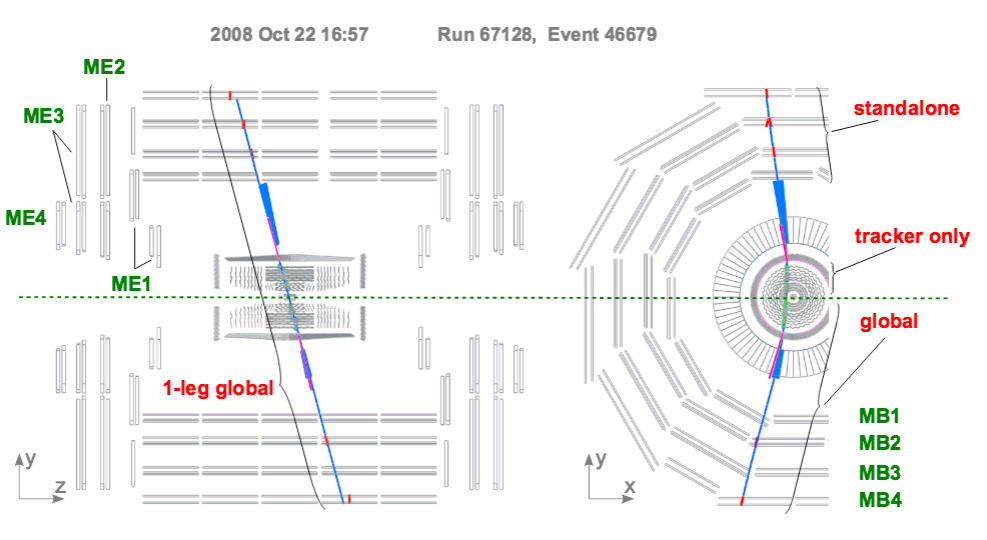
\includegraphics[width=0.99\textwidth]{Chapters/xLHCMS/CosmicMuons.png}
\caption{Event display of a cosmic muon passing through the CMS
  detector. Standalone and global trajectories are
  outlined. From~\cite{Chatrchyan:2009ae}.} 
% Personal compilation for Scomparin~\cite{scomparinlhcp2014}.}
\label{fig:cosmicmuon}
\end{center}
\end{figure}

\subsection{Global muons}
\label{sec:GLB}
The Global muon object (GLB) extends the muon trajectories to include
silicon tracker hits. From the standalone muon previously obtained,
the trajectory is extrapolated to the outer tracker layers. The
outcome of this extrapolation is the definition of a region of
interest in the trackers' sensitive areas where the track reconstruction is
performed.
\\
Within the region of interest, initial track candidates for the matching
with the extrapolated STA are built from pairs of reconstructed
tracker hits originating from two different tracking layers. All
combinations of pixel layers and double sided silicon strips are used
in the pairing. The track reconstruction algorithm, based on the
Kalman-filter technique,
\begin{itemize}

\item[-] builds tracks in the region of interest from
pixel-seeded pattern recognition,
\item[-] cleans the built tracks by resolving
position and momentum ambiguities,
\item[-] refits the obtained
trajectory.

\end{itemize} Starting from the innermost layer, the trajectory is
propagated to the above layers, and the measurement improves at each
iteration. The best $\chi^{2}$ for the track fit is retained if
multiple tracks are compatible. Finally, all reconstructed tracks are
fitted again without any beamspot constraint, and using STA muon
hits. The GLB muon candidates are further cleaned by a $\chi^{2}$ cut
on this global fit. The candidates with high global $\chi^{2}$ are
discarded. The remaining trajectories undergo an additional fit, excluding
muon chamber hits and segments with high  $\chi^{2}$ values, and using
only silicon tracker fits plus the innermost muon station
measurements. The  $\chi^{2}$ probability of the new fit is compared
with the tracker only trajectory, which helps detecting energy loss
before the muon reached the first muon station. This procedure ensures
a good momentum reconstruction up to \pt$\sim$1 \TeVc.

An example of GLB muon can be found in Figure~\ref{fig:cosmicmuon},
where an event display of a cosmic muon passing through CMS is
shown. This event, compared to collision events, has the particularity
of having no backgrounds, and a trajectory very displaced from the
beamspot.
\begin{figure}[!htb]
  \begin{center}
    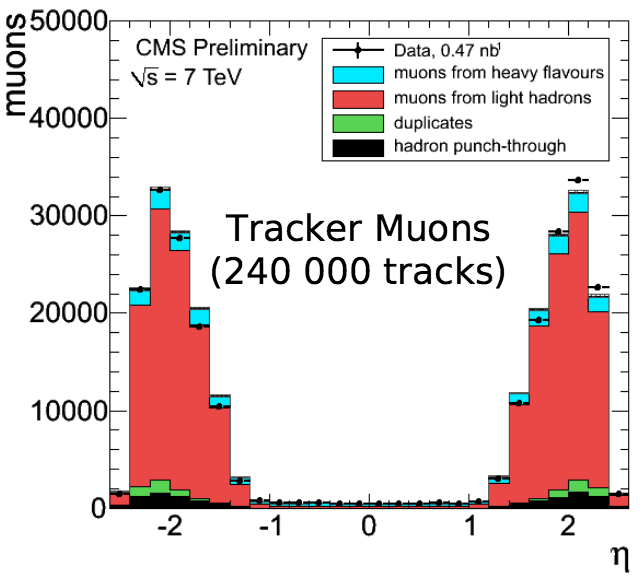
\includegraphics[width=0.45\textwidth]{Chapters/xLHCMS/TrkMuon_eta.png}
    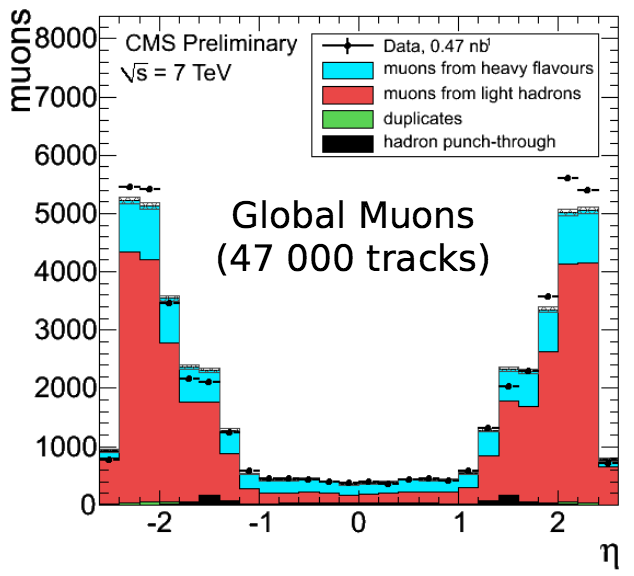
\includegraphics[width=0.45\textwidth]{Chapters/xLHCMS/GlbMuon_eta.png}


    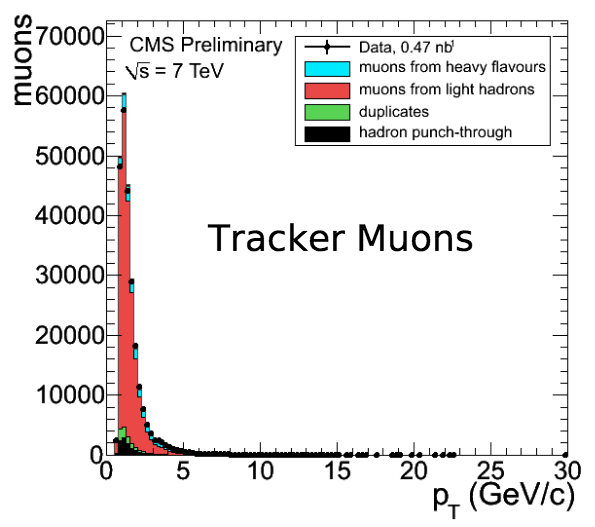
\includegraphics[width=0.45\textwidth]{Chapters/xLHCMS/TrkMuon_pt.png}
    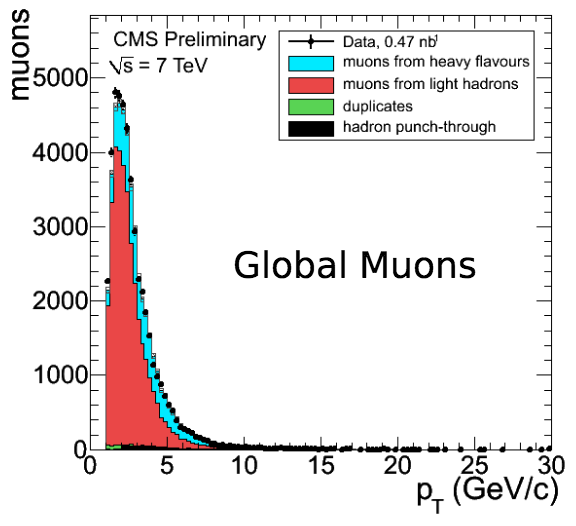
\includegraphics[width=0.45\textwidth]{Chapters/xLHCMS/GlbMuon_pt.png}

    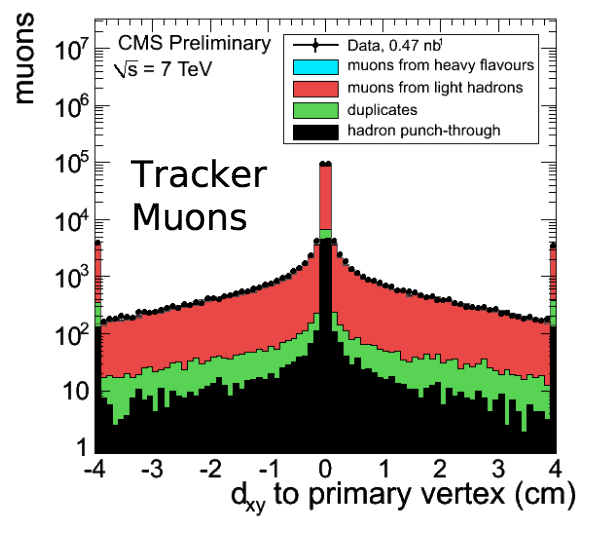
\includegraphics[width=0.45\textwidth]{Chapters/xLHCMS/TrkMuon_dxy.png}
    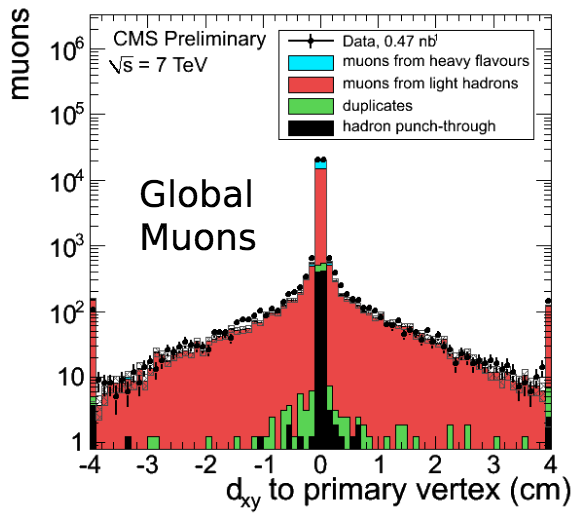
\includegraphics[width=0.45\textwidth]{Chapters/xLHCMS/GlbMuon_dxy.png}
    \caption{Kinematic distributions for tracker muons (left) and global
      muons (right), in early 7 \TeV\ $pp$ data. Top: pseudorapidity
      distributions.  Middle: \pt\ distributions. Bottom:
      distance to the primary vertex in the $x-y$ plane~\cite{muo}.} 
    \label{fig:muonpogplot}
  \end{center}
\end{figure}

\subsection{Tracker muons}
\label{sec:TRK}

An approach complementary to the GLB muon reconstruction consists
in considering all tracker tracks to be potential muon candidates and
in checking this hypothesis by looking for compatible signatures in
the calorimeters and in the first layer of muon systems. The reconstructed tracks
with \pt\ above 2.5 \GeVc compatible with at least one hit
in one of the inner muon stations, are kept for further refitting
following the procedure described above. This approach is famous for
low \pt\ muons in $pp$ data, but would be unaffordable given the CPU
time it would require to run over all tracker tracks in heavy ion collisions.
\\
A comparison between global and tracker muons is possible, and was
done with early 2010 $pp$ data at \s\ = 2.76 \TeV~\cite{muo}. The Muon
Physics Object Group of CMS (Muon POG)~\cite{muonpog} is responsible of maintaining
the reconstruction codes and provides useful guidelines on how to
reconstruct muons in CMS. The Muon POG is also responsible of
preparing performance studies on muon identification and
reconstruction for every data taking period (Run1,
Run2, etc.)~\cite{Chatrchyan:2013sba}~\cite{CMS-PAS-MUO-10-002}. In
Figure~\ref{fig:muonpogplot}, some basic kinematic distributions comparing
7 \TeV\ tracker and global muons are compared. We can see that in the
three distributions ($\eta$, $\pt$, $d_{xy}$), the tracker muon
data is consistently more populated by light flavour (simulated) muon
decays, duplicates, and hadron punch through. The global muons,
although comparable, seem to perform better when one wants to
discriminate easily the light flavour muons from heavy flavour
muons. These plots were made with no specific quality requirement; we
can understand that tracker muons will perform well as long as some
additional offline cuts on the track quality are met. 


\subsection{Tracking in heavy ion collisions}
\label{sec:hireco}
Specific
reconstruction and tracking algorithms are required to build muon
trajectories in heavy ion collisions. Furthermore, the kinematic
region of interest for muons in heavy ion physics is mostly located at
low \pt, where charmonia, bottomonia and open heavy flavour are
abundantly produced. However, the relatively low luminosity at which the
LHC delivers PbPb collisions to the detectors (cf. Section~\ref{sec:HiRates}) makes it possible to
reconstruct a large fraction of the heavy ion event, without burning
the pixel detector and without losing performance dramatically in all
of the subdetectors.


The track reconstruction sequence is modified in heavy ion collisions from what
was presented in Section~\ref{sec:GLB}, in the following way~\cite{Denterria:2007xr}:

\begin{itemize}
\item[-] Instead of building a pixel hit start pair and extrapolate
  along a rectangular region of interest using pattern recognition,
  the builder extrapolates the trajectory helix to the transverse plane
  region where the next layer is, forming a smaller circular area to
  pick tracker hits into. This is the \textit{modified hit triplet finding};
\item[-] \textit{triplet cleaning}: if one of the hits in the triplet is not compatible with the
  incidence angle of the track, the triplet is discarded;
\end{itemize}

% Figure~\ref{fig:hitracking} shows how the occupancy in pixel and
% silicon tracker layers perform in PbPb simulations. 

The muon and track reconstruction strategies in heavy ion collisions have improved in 2012, leading to a
re-reconstruction of the PbPb 2011 run. 

The 2011 track reconstruction consisted of three iterations of the
process mentioned in Section~\ref{sec:GLB}. The first two iterations
began with triplet seeds, while the third formed tracks using a
very limited subset of doublet seeds. 


In the current muon
reconstruction, the tracking algorithm is called Regional Iterative
Tracking (RegIT). RegIt doubled the number of iterations, restricted in a
cone around the STA muon extrapolation to beamspot, to minimise the
computing time. 

To further optimise the tracker reconstruction in
PbPb, e.g. in the case of displaced muons (non-prompt \Jpsi), two
additional steps were added to further improve the reconstruction
efficiency: first, a displaced triplet step was added by removing the beamspot
constraint. Second, the triplet seed for tracking, usually based on
pixel hits, was allowed to pick starting hits in the silicon tracker,
making the seed a \textit{mixed triplet seed} (Pixel+strip triplet).


These two improvements have an effect of approximately 15\% on each
muon in a dimuon pair, when integrating over position variables
($r,\phi$). A similar strategy is applied in high pile-up $pp$ data,
and the efficiency improvement is clear in tracks highly distant from
the beamspot, starting from the fourth tracking iteration and above~\cite{pileup}.



\subsection{Muon selection}
% \subsection{heavy-ion event reconstruction} %RegIT
\label{sec:muonID}

In the previous subsection we have seen what muon types are
available. Especially, it was argued in Figure~\ref{fig:muonpogplot}
that the tracker muons, for example, can be overwhelmed by light
flavour muons, or duplicates. To the contrary, global muons, whose
reconstruction sequence initiates in the muon chamber and propagates
to the inner tracker, with a refitting including the primary vertex,
can gain better discriminative power for heavy flavour and relatively
high-\pt\ muons (i.e. below the \TeV\ scale, roughly). 


Since the analysis envisioned in this Thesis aims at performing the
same signal extraction, $\PgU \to \mu\mu$ in two samples with very
different tracker occupancy, a safe strategy must be adopted, to
ensure high reconstruction efficiency and reasonable processing time
(of the order of 5 seconds for central PbPb events). Global muons were
used, since tracker based muons are not affordable starting from
mid-central PbPb events.


While doing the GLB muon reconstruction, the code stores the
information relative to the number of hits in the muon chambers, the
number of pixel hits and tracker layers in
the tracker systems, as well as the info from the global track
refitting (total number of hits, reduced $\chi^{2}$ of global
fit). These could be further used to discard low-purity
tracks. Additionally, the fitted tracker track distance from the
primary interaction vertex is computed and can be used to remove muons
originating from long lived particle decays ($\pi, K$, ...) as well as
cosmic rays.


The list of available~\textit{identification} variables is detailed
below, along with the cut applied in our $pp$ and PbPb analyses,
placed in parenthesis and in bold. This set of cuts is recommended for
most analyses using low \pt\ muons in CMS using the software developed
at the time of PbPb data\footnote{CMSSW\_4\_4\_X}
re-reconstruction (2012): 
\begin{itemize}
\item[1] Tracker based quantities:
  \begin{itemize}
  \item[-] Number of valid pixel hits (\textbf{$\geq$ 1}): final number of pixel hits
    from the total tracker track fit (some can be discarded, from
    the second iteration of the Kalman-filter method). A cut on this
    variable would remove muons from decays in flight;
  \item[-] Number of silicon tracker layers with measurement  (\textbf{$\geq$ 10}). To
    guarantee a good \pt\ measurement, for which some minimal number
    of measurement points in the tracker is needed.
    Also suppresses muons from decays in flight;
  \item[-] $d_{xy}$  (\textbf{$<$ 3 cm}): tracker track transverse impact parameter,
    i.e. closest distance in the $x-y$ plane to the primary vertex. To
    suppress cosmic muons and further suppress muons from decays in
    flight;
  \item[-] $d_{z}$  (\textbf{$<$ 15 cm}):  longitudinal distance of the tracker track with
    respect to the primary vertex. To further suppress cosmic muons,
    muons from decays in flight and tracks from pile-up;
  \item[-] reduced $\chi^{2}$ of the muon track  (\textbf{$<$ 4}): to cut the badly
    reconstructed tracks (duplicates, punchtrough, long-lived);
  \item[-] tracker arbitration  (\textbf{true}): if there exist an ambiguity in the
    track-muon segment matching. The one arbitrated track has the closest geometric
    coordinates to the muon track (i.e. within three centimeters) when
    extrapolated to the muon station;
  \item[-] \verb?TMOneStationTight?  (\textbf{not used}): Tracker track matched with at
    least one muon segment in any station in three standard deviations
    of the size of the STA muon track, in the $x-y$ plane. To resolve
    ambiguities when first muon station is shared by several tracks.
  \end{itemize}
\item[2] Global muon quantities:
  \begin{itemize}
  \item[-] \verb?isGlobal()?  (\textbf{true}): requires the existence of a global
    muon. To remove empty muon station events;
  \item[-] number of valid muon chamber hits  (\textbf{not used}):
    removes a good part of the hadronic punchthrough; 
  \item[-] reduced $\chi^{2}$ of the global muon trajectory  (\textbf{$<$ 10}): To
    suppress hadronic punch-through and muons from decays in flight. 
  \end{itemize}
\end{itemize}



\vspace{0.5em}
\begin{center}
  \fbox{
    \parbox{0.9\textwidth}
    {\textsf {In this section, the procedures to reconstruct muons
        passing the trigger requirements were outlined. We have seen
        that the $pp$ and PbPb reconstruction algotrithms involve
        information from muon subdetectors to first reconstruct a
        \textit{standalone} muon track, then propagated inwards to try
        to match it with a tracker track. The muon identification is
        meant to remove at the analysis step (offline) muons being
        poorly reconstructed, and enrich our sample in muons of good
        resolution. The muon selection used in further Chapters for
        yield extraction and efficiency corrections retains
        \textit{global} muons. The reconstruction efficiency of these
        muons will be covered in Chapter~\ref{chap:aCorrection}.}}} 
\end{center}

\clearpage
\section{Event selection and centrality}
\label{sec:evtsel}
In this section we will see how the global event selection is applied
to our muon sample. This will help extract the correct normalisations
in order to compute an \PgU\ production rate compatible with a cross
section times branching ratio.
\subsection{\texorpdfstring{$pp$}{pp} luminosity}
\label{sec:pplumi}
The instantaneous luminosity $\mathcal{L}_{\textrm{inst.}}$, encountered previously when discussing
trigger rates, is defined in Equation~\ref{eq:lumicon}:

\begin{equation}
 R = \mathcal{L}_{\textrm{inst.}}\sigma,
\label{eq:lumicon}
\end{equation}

where $R$ is the rate of a physical process, corresponding to a
production cross section $\sigma$. The integrated luminosity is the
integral of $\mathcal{L}_{\textrm{inst.}}$ over the whole data taking
time.


Since the LHC settings are not optimal to measure the total $pp$ cross
section with precision~\cite{Bayatian:2006zz}, one cannot rely on the
above formula to compute the luminosity recorded over a full physics
run, without making an assumption on the total $pp$ interaction cross
section, which is dependent on the centre-of-mass energy.

However, the \textit{minimum bias} requirement to select events
originating from a hard diffusion, i.e. removing photo production and
double pomeron physics, as well as other elastic processes, is
nowadays done in CMS by requesting a minimal number of energy deposits
in the Hadron Forward (HF) detectors. Our requirement is to record at
least one tower with energy above 3 \GeV\ on each side of the HF, when
performing $pp$ collisions. The counted number of events can be used
to extract a luminosity.


The validation procedure of this number requires to define a set of
good running times (i.e. when the high voltage is on and all
subdetectors are running well). In this way the HF detector also
fulfills a role of luminometer. It can also be cross checked by the
LHC accelerator team by performing Van der Meer scans upstream of the
machine. The Van der Meer procedure is to scan the transverse profile
of proton beams; by doing so, and knowing the LHC filling scheme and
the number of circulating protons, allows to determine an absolute
luminosity scale, which can in turn be used to calibrate the HF
luminometer.

In 2013, the certified $pp$ integrated luminosity recorded during the CMS run at
\s\ = 2.76 \TeV\ is:

\begin{equation}
\mathcal{L}_{pp} = (5.4 \pm 0.2)\; \invpb.
\label{eq:lumiCMS}
\end{equation}
\subsection{Minimum bias event selection in PbPb collisions}
\label{sec:minbias}
If one wants to compute a cross section in PbPb collisions, one would need an
equivalent measurement as the $pp$ luminosity measurement of
Equation~\ref{eq:lumiCMS}. The $pp$ luminosity is dependent on the
total cross section for proton-proton interaction at the
centre-of-mass energy of \s\ = 2.76 \TeV. 
\\
Unfortunately, the total PbPb cross section (inelastic plus elastic scattering cross
section) is not known, and one would need a workaround,
namely, an estimate of the total number of recorded hadronic
interaction events. This number has to be counted with the total PbPb
run data: it is not the number of events producing dimuons. 

Additional care has to be taken in the event selection of the PbPb sample:
since the Pb ions carry 82 positive electric charges each, it is much
more probable that long range electromagnetic interactions occur
between the Pb ions. Furthermore, any beam-gas interaction should be
removed, both from the event counting and the dimuon sample. For this
reason, the following event \textit{minimum bias} selection cuts are
applied to the overall PbPb dataset:


\begin{itemize}

\item[-] Beam-halo muons (accelerator-induced particles that travel
  along the beam line and can be detected at any height $r$ in both
  endcaps~\cite{beamhalo}) are removed by requesting that dimuon triggers are in time with
  beam-scintillator counters used for beam crossing precise timing,
  placed at the ends of both HF sides;
\item[-] Ultraperipheral collisions (induced by the electric
  charges in presence, for example $\gamma$~Pb~$\to \mu^{+}\mu^{-}$~Pb) and
  beam-gas events are vetoed by an offline filter requesting the
  firing of three HF towers on each side of the
  interaction point, with a total deposited energy of more than 3
  \GeV, in coincidence with the trigger dimuon event;
\item[-] A reconstructed vertex of at least two tracks of \pt above 75
  \MeVc\ should be found, consistent with the transverse beam spot
  position and the expected collisions region along the $z$-axis;
\item[-] Further rejection of beam-gas and beam scraping events is
  done by requesting the longitudinal length of pixel clusters
  to be compatible with particles originating from the primary
  vertex. This selection proved efficient since the first publication
  on pseudorapidity and \pt\ distributions of charged particles in 7
  \TeV\ $pp$ collisions~\cite{ppmult}. This cut is placed along the red
  line visible on Figure~\ref{fig:eventselectioncuts} (left);

\end{itemize}

This selection ensures a tight correlation between the sum energy
recorded by the two HF calorimeters and the number of pixel hits. The
correlation can be seen on Figure~\ref{fig:eventselectioncuts}
(right). It furthermore indicates that the HF energy sum can be later
used as a classification variable for the `centrality' of the
collision, defined below.


\begin{figure}[!htb]
  \begin{center}
    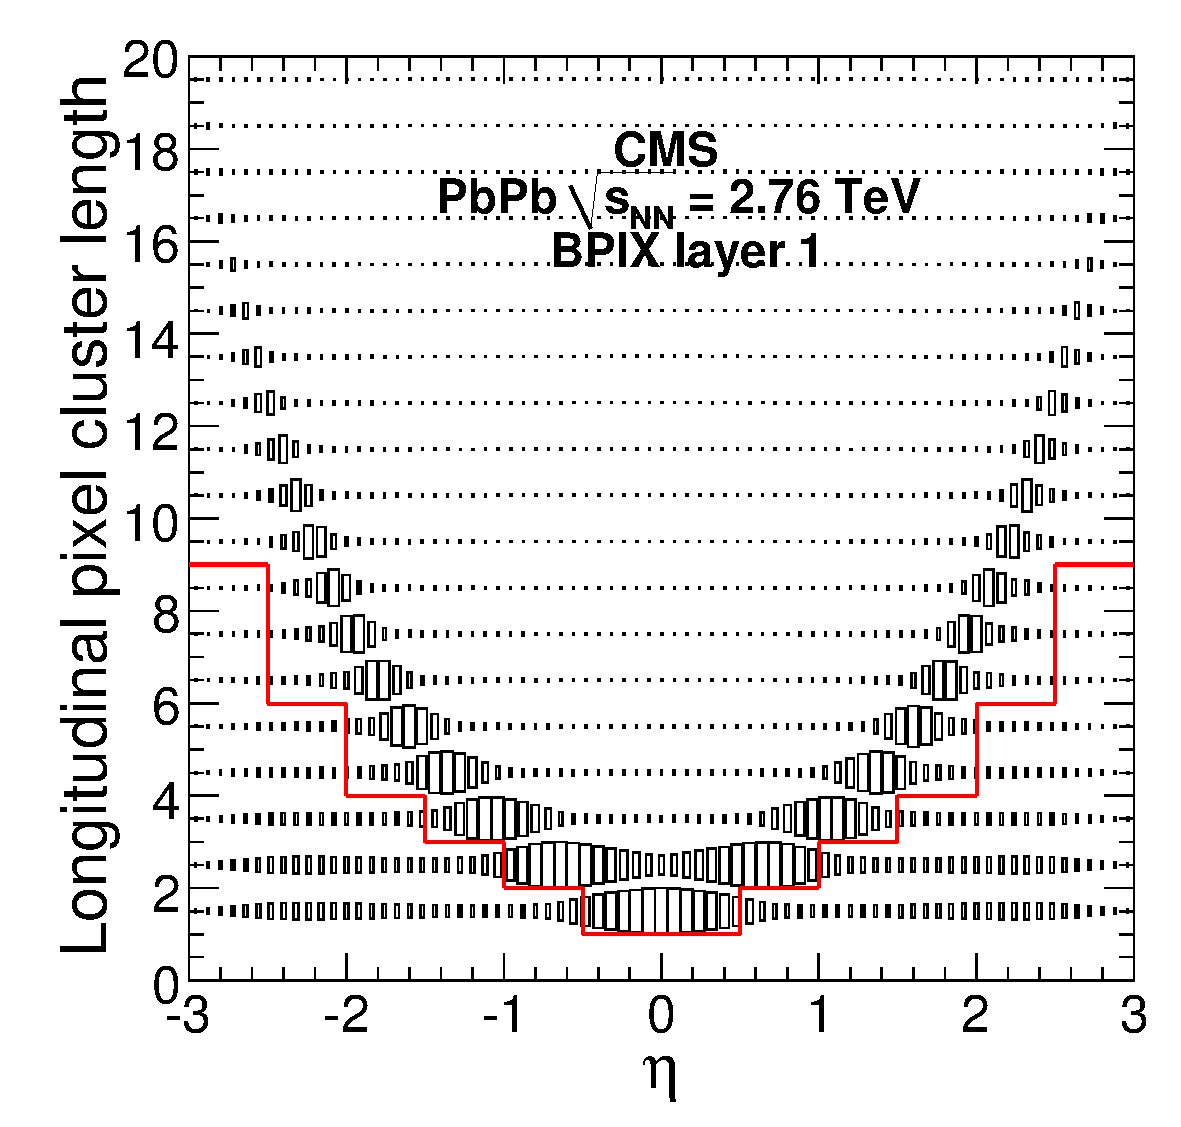
\includegraphics[width=0.43\textwidth]{Chapters/xLHCMS/HIN_10_001_Fig2b.pdf}
    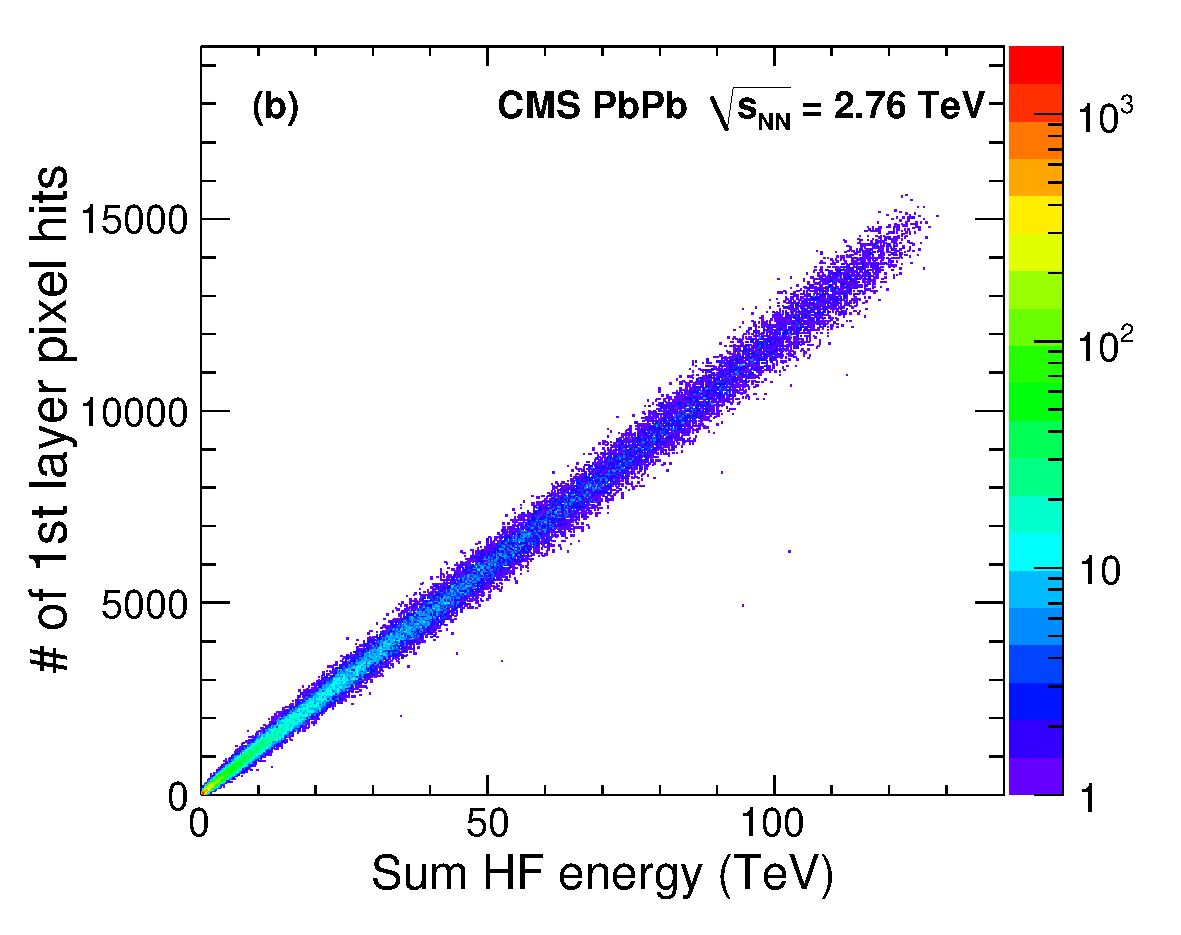
\includegraphics[width=0.53\textwidth]{Chapters/xLHCMS/PixelHits_vs_sumHFenergy_collisions.pdf}
    \caption{Global PbPb event selection performance-oriented
      plots. Left: Pixel-cluster length along the beam direction in
      units of pixel cells for hits from the first layer of the pixel
      detector, as a function pseudorapidity, after the rest of the
      event selection. The solid red line shows the selection on the
      minimum cluster length used~\cite{pbpbmult} Right: Correlation between the number of pixel
      hits and HF total energy for a single run containing 60 000 minimum
    bias events after the selections described in Section~\ref{sec:minbias}~\cite{Chatrchyan:2011sx}.} 
    \label{fig:eventselectioncuts}
  \end{center}
\end{figure}


With this selection, the total number of events recorded in 2011
passing the cuts is \NMB$_{\rm raw}$, the raw \textit{number of
  minimum bias events}, 
which is equal to: 
\begin{equation}
\NMB\,_{\rm raw} =  1\,126\,653\,312
\end{equation}
The minimum bias selection efficiency, i.e. the fraction of the total
inelastic PbPb cross section covered by this selection, was estimated
in~\cite{Chatrchyan:2011sx} to 97 $\pm$ 3 \%.

The corrected number of minimum bias events, $\NMB =
1\,161\,498\,260$, is used in the normalisation of the PbPb sample, to
get a number close to the actual \PgU\ cross section. In the following
subsection we will see how the dimensionality of a cross section is
recovered, and how the PbPb events are split in centrality classes.
%
%


\subsection{Centrality}
\label{sec:centrality}


The centrality of a nucleus-nucleus collision accounts for the overlap
of the two nuclei at the moment of their collision. If the overlap is
maximal, the maximum number of nucleons will participate in the
collision: in the case of Pb ions, it is 208$\times$2 = 416. The most
central events are the ones close to this number of participating (or
\textit{wounded}) nucleons.


In a collider experiment, we cannot have a direct access to the exact
number of nucleons colliding in any Pb-Pb interaction. One
experimental handle would be the total event multiplicity for example,
as the collision events with large impact parameter (i.e., the most
\textit{peripheral} events) produce very few
particles, while the central ones with small impact parameter can
produce many more particles.


We also know from $pp$ interactions at recent and past collider energies that
the multiplicity of particles produced in a head on $pp$ scattering
can be larger than the number of particles in the initial state (that
is 2), and can vary event by event. Counting the number of
final state particles would then be helpless, especially in the very high
density regime reached in PbPb collisions as \snn\ = 2.76 \TeV.

However, we have seen in Section~\ref{sec:minbias} that after the
minimum bias selection, the multiplicity of pixel hits in the first layer, seen in
Figure~\ref{fig:eventselectioncuts}, correlates very well with
the sum of energy accumulated in the forward hadron calorimeters, with
only few events deviating significantly\footnote{To verify this, the
  electronic version of Figure~\ref{fig:eventselectioncuts} (right) may work
  best, as the binning of the 2D plot may be too small to notice
  deviations in the printed version.}.


The distribution of this total forward energy was then used to divide
the event sample into forty centrality classes, each representing
2.5\% of the total nucleus nucleus interaction cross section. The
sorting of the $\sum{}E_{T}^{HF}$ distribution in centrality classes is
shown in Figure~\ref{fig:hfet}.



\begin{figure}[!htb]
  \begin{center}
    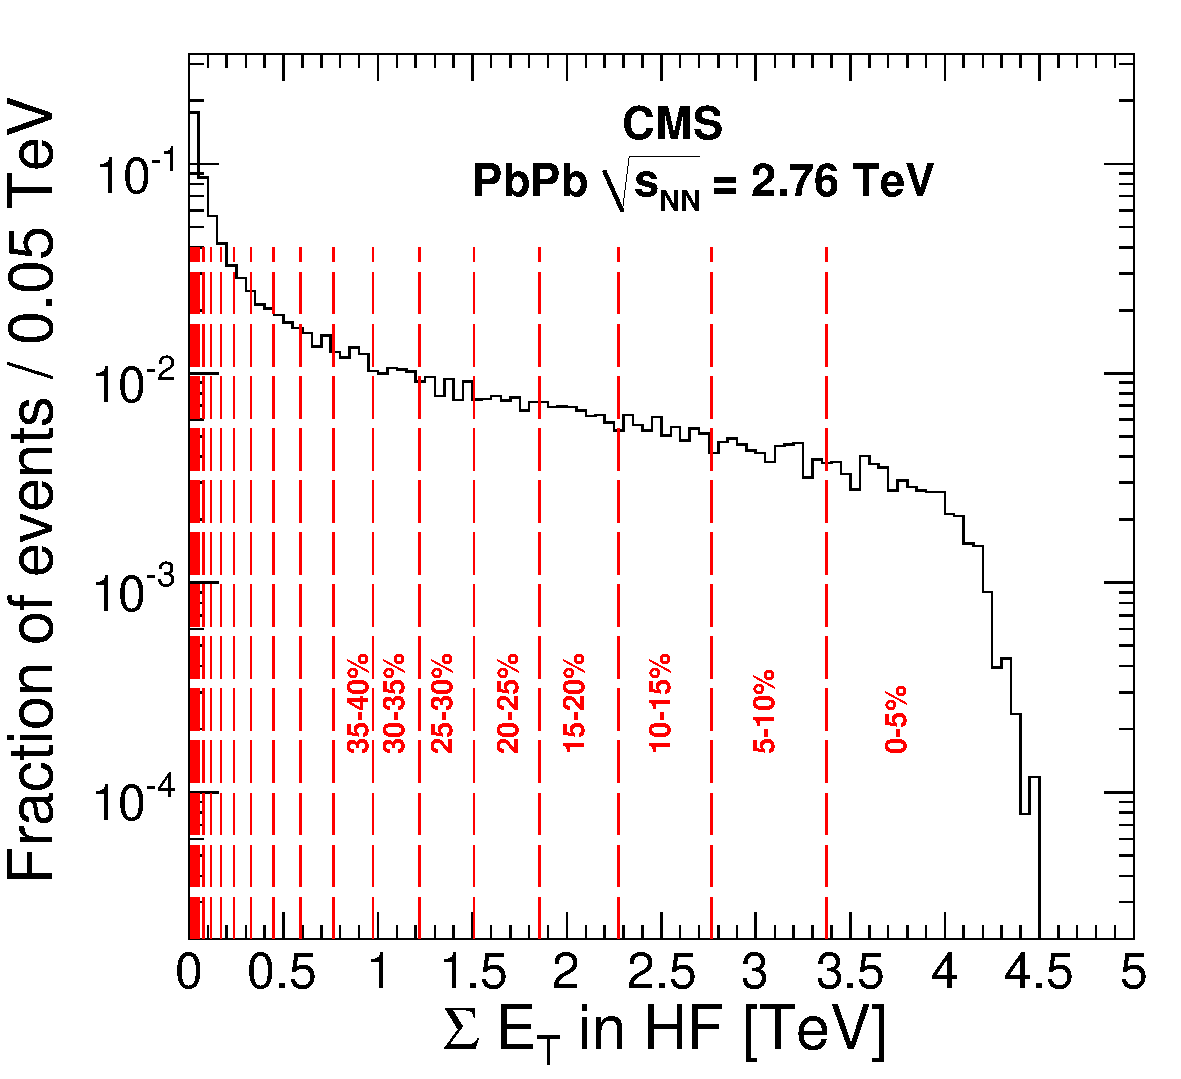
\includegraphics[width=0.7\textwidth]{Chapters/xLHCMS/HIN_10_001_Fig1.pdf}
    \caption{Centrality sampling on the total HF energy recorded in
      PbPb collisions at \snn\ = 2.76 \TeV, from~\cite{pbpbmult}.} 
    \label{fig:hfet}
  \end{center}
\end{figure}




Simulations can be used to correlate the defined centrality to the
impact parameter $b$ between the two nuclei, and to other properties of the
collisions. The main quantities of interest are:

\begin{itemize}
\item[-] \Npart, the total number of nucleons that have experienced at
  least one inelastic scattering in the AA collision. This number
  cannot exceed 2$\times$A, with A = 208 for Pb nuclei;
\item[-] \Ncoll, the total number of nucleon-nucleon scatterings in
  the nucleus-nucleus collision. This number can very well exceed
  \Npart\ or 2 $\times$ A, depending on the impact parameter: for example, in the
  10\% most central events, we have $b$ = [3.4 $\pm$ 0.1 (RMS = 1.2)]
  fm, $\langle \Npart \rangle$ =  355 $\pm$ 3 (RMS = 33), and $\langle
  \Ncoll \rangle$ =  1484 $\pm$ 120 (RMS = 241);
\item[-] \TAA, the nuclear overlap function, which has units of a
  cross section. \TAA\ is equal to \Ncoll\ divided by the elementary
  nucleon-nucleon cross section and can be interpreted as the
  equivalent integrated luminosity per heavy ion collision, in a given
  centrality range. For Pb ions at 2.76 \TeV, the centrality averaged
  value is \TAA\ = [5.66 $\pm$ 0.35 (RMS = 7.54)] mb$^{-1}$;
\end{itemize}


The average values and variances for $b$, \Npart, \Ncoll\ and \TAA\ are
obtained in a calculation based on a Glauber model, in which it is
assumed that nucleons follow straight line trajectories in the PbPb
collision~\cite{Miller:2007ri}. The distribution of nucleons inside
each nucleus is assumed to follow a Woods-Saxon
distribution~\cite{de1974nuclear}. The resulting number of
nucleon-nucleon interactions depends on how close the nucleons need to
be in the transverse plane of the PbPb collision for a nucleon-nucleon
scattering to occur; Based on fits to the available total and elastic
cross sections in proton-proton and proton-antiproton
collisions~\cite{Agashe:2014kda}, the elementary nucleon-nucleon cross section
is taken to be $\sigma_{\rm inel}$(NN) = 64 $\pm$ 5 mb. 
%HIN_10_001_Fig1.pdf


The values for $b$, \Npart\ and \Ncoll, in fine 2.5\% bins are
reported in Appendix~\ref{sCentrality}. The \Npart\ and \TAA\ values used in this
analysis are however presented in larger bins in Table~\ref{tab:glauber},
corresponding to the centrality bins used in Chapter~\ref{chap:ayield}.

% In the \PgU\ measurement in PbPb, as for many hard probes measured in
% heavy ions, it is important to realise that the 
Dimuon triggered
events such as \Jpsi\ or \PgU\ decays are not distributed evenly among centrality classes. In fact,
dimuon events originate from hard parton-parton scatterings, that do
not conform to the centrality distribution of soft events. The soft
particle rate (of $\pi, K$ for example) is proportional to \Npart, the
number of participating nucleons in the collision, while harder probes
(such as open heavy flavour, jets, quarkonia and electroweak bosons)
are produced proportional to \Ncoll, which increases faster than
\Npart\ with increasing centrality. This can be seen in
Figure~\ref{fig:centrality10-006}, where the centrality distribution
of minimum bias triggered events is compared to dimuon triggered
events.

\begin{figure}[!htb]
  \begin{center}
    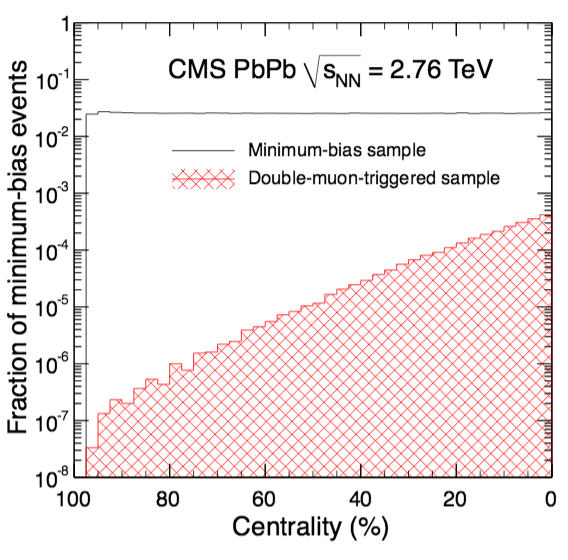
\includegraphics[width=0.7\textwidth]{Chapters/xLHCMS/Centrality10-006.png}
    \caption{Centrality distribution of events passing minimum bias
      triggers compared to dimuon triggered events, in bins of 2.5\%~\cite{torsten}.} 
    \label{fig:centrality10-006}
  \end{center}
\end{figure}




\begin{table}[htbp]
  \begin{center}
    
    \begin{tabular}{rcccccc}
      \hline\vspace{0.1em}
      % ~ & \multicolumn{2}{c}{$\Npart$} & \multicolumn{2}{c}{$\TAA$ (mb$^{-1}$)}\\
      Centrality (\%) & \Npart\ & \TAA~(mb$^{-1}$) \\\hline
      0--5	& 381  & 25.9 $\pm$ 1.1 \\
      5--10	& 329  & 20.5 $\pm$ 0.9 \\
      10--20	& 261 & 14.5 $\pm$ 0.76 \\
      20--30	& 187 & 8.78 $\pm$ 0.58 \\
      30--40	& 130 & 5.09 $\pm$ 0.43 \\
      40--50	& 86.3 & 2.75 $\pm$ 0.30 \\ \hline
      50--70    & 42.0 & 0.985 $\pm$ 0.145 \\
      70--100   & 8.75 & 0.130 $\pm$ 0.020 \\ \hline
      50--100	& 22.1 & 0.486 $\pm$ 0.073 \\ \hline
      0--100	& 113 & 5.66 $\pm$ 0.35 \\ \hline
    \end{tabular}
  \end{center}
  \caption{Average values of the number of
      participating nucleons (\Npart) and of the nuclear overlap function
      (\TAA) in PbPb collisions, with the centrality bins used in this
      analysis~\cite{Chatrchyan:2011sx}.}
    \label{tab:glauber}
\end{table}



\vspace{0.5em}
\begin{center}
  \fbox{
    \parbox{0.9\textwidth}
    {\textsf {In this section we have seen how hadronic events are
        selected in $pp$ and PbPb collisions, which led us to introduce the
        integrated luminosity used in the $pp$ sample. One measure of
        the total number of hadronic (\textit{minimum bias}) events in
      PbPb collisions is presented. The centrality of the collision has been
      defined, and is indispensable to estimate the amount suppression seen by
      quarkonia at increasing energy densities in nuclear matter. This
    closes the chapter of event selection and muon selection,
    providing us with all the tools needed for the study of \PgU\ yields
  in data in the next part.}}} 
\end{center}



% \section{The global muon object}
% \subsection{Standalone muons}
% \subsection{Tracker muons}
% \section{Performance of the Muon reconstruction}
% subsection{}

